% Provenance (never printed): old terminale S material on the Earth's internal
% heat (geothermal gradient and heat flow, radioactive heat production,
% conduction and convection, mantle convection, geothermal energy). Owner
% (Sync 0/1): heat flow, radiogenic heat production, secular cooling, thermal
% and mantle convection (recall the convection cell of Book 1 g8 first),
% geothermal energy. Geotherm and geothermal gradient are g11.03's; radioactivity,
% half-life, decay law and thermal conductivity are physics' (thermal
% conductivity used as "the rock's thermal conductivity k", never defined);
% hotspot track and plume g11.04's. Figures: figdata/grade-12/internal_heat.py.
\chapter{O calor interno da Terra}\label{ch:g12:internal-heat}

Entre 1987 e 1995, perto do vilarejo de Windischeschenbach, na Baviera,
geólogos perfuraram um furo de \qty{9101}{m} de profundidade na \omterm{def:g12:continental-crust:continental-crust}{crosta
continental}. No fundo, a rocha estava a cerca de \qty{265}{\celsius}, quente
demais para perfurar mais fundo.
% ledger: gfz:ktb, gfz:ktb30

De cerca de \qty{10}{\celsius} na superfície a \qty{265}{\celsius} a
\qty{9.1}{km}, a temperatura sobe cerca de \qty{28}{\celsius} por
quilômetro, um valor típico. Em toda parte da Terra, fica mais quente para
baixo, por isso o calor sai da Terra o tempo todo. Este capítulo mede esse
fluxo, pergunta de onde vem o calor, e mostra como ele se desloca.
% values: ktb_gradient 28.0 (internal_heat.py, surface temperature taken as 10 degC); ledger: gfz:ktb (gradient about 28 K/km)

\begin{recall}
A \omterm{def:g11:lithosphere-asthenosphere:geotherm}{geoterma} é a curva da temperatura em função da profundidade sob um lugar,
e o \omterm{def:g11:lithosphere-asthenosphere:geotherm}{gradiente geotérmico} a subida da temperatura por quilômetro; os furos de
sondagem medem de 25 a \qty{30}{\celsius} por quilômetro perto da superfície
(\cref{ch:g11:lithosphere-asthenosphere}). Alguns átomos são radioativos:
eles decaem ao acaso, o número dos que restam caindo pela metade a cada
meia-vida, e cada decaimento libera energia, que acaba virando calor (os
livros de física). Uma célula de convecção é um circuito de fluido aquecido
por baixo, que sobe, se espalha, esfria e desce (Livro 1, 8º ano). Num ponto
quente, uma placa se move sobre uma pluma de manto quente
(\cref{ch:g11:plate-motions}).
\end{recall}
% ledger: usgs:gradient-29 (Book 1 row)

\section{Gradiente e fluxo de calor}

\begin{definition}[Fluxo de calor]\label{def:g12:internal-heat:heat-flow}
O \emph{fluxo de calor}\index{fluxo de calor} (ou fluxo térmico) num lugar é
a potência que sai do interior da Terra através de cada metro quadrado da
sua superfície ali. Ele se mede em miliwatts por metro quadrado
(\unit{mW/m^2}).
\end{definition}
% ledger: b2dd10:continents

O calor flui do quente para o frio, e quanto mais íngreme o gradiente de
temperatura, mais depressa ele flui. Quanto flui depende também da rocha:
cada rocha tem uma condutividade térmica $k$, em watts por metro por kelvin,
que os livros de física definem.

\begin{proposition}[Fluxo de calor e gradiente]\label{prop:g12:internal-heat:fourier}
Através de uma rocha de condutividade térmica $k$ na qual a temperatura sobe
com a profundidade segundo um gradiente $G$ (em kelvins por metro), o \omterm{def:g12:internal-heat:heat-flow}{fluxo
de calor} para cima, em direção à superfície, é
\[
  q = k\,G .
\]
\end{proposition}

Essa lei da condução, devida a Fourier, é admitida aqui; os livros de física
a demonstram numa forma geral.

\begin{method}[Um fluxo de calor a partir de um furo de sondagem]\label{met:g12:internal-heat:borehole}
\begin{enumerate}
  \item Meça a temperatura a várias profundidades de um furo de sondagem,
        depois que o furo teve tempo de voltar à temperatura da rocha.
  \item Represente a temperatura em função da profundidade e tome a
        inclinação: o gradiente $G$, convertido em kelvins por metro.
  \item Meça a condutividade $k$ da rocha em testemunhos, no laboratório.
  \item Multiplique: $q = kG$, em \unit{W/m^2}, e depois converta em
        \unit{mW/m^2}.
\end{enumerate}
\end{method}

\begin{example}[Um furo de sondagem no granito]\label{ex:g12:internal-heat:borehole}
Um furo de sondagem num granito de condutividade \qty{2.72}{W/(m.K)} mede um
gradiente de \qty{29}{\celsius} por quilômetro, isto é, \qty{0.029}{K/m}.
Então $q = 2.72 \times 0.029 \approx \qty{0.079}{W/m^2}$, cerca de
\qty{79}{mW/m^2}.
\end{example}
% ledger: roy:conductivity (granitic layer 6.5 mcal/(cm s degC) = 2.72 W/m/K), usgs:gradient-29 (Book 1 row)
% values: borehole_q_mW 78.9 (internal_heat.py)

Mais de 38\,000 medições desse tipo foram combinadas num mapa da Terra
inteira. Os continentes perdem em média \qty{70.9}{mW/m^2}, o fundo oceânico
\qty{105.4}{mW/m^2}; sobre toda a superfície, \qty{91.6}{mW/m^2}.
Multiplicado pela área da Terra, \qty{5.101e14}{m^2}, o total é
\[
  0.0916 \times \num{5.101e14} \approx \qty{4.67e13}{W} = \qty{46.7}{TW},
\]
cerca de 47 terawatts, com uma margem de 2.
% ledger: b2dd10:continents, b2dd10:half-space (47 +- 2 TW, 38,347 measurements)

O fundo oceânico perde mais onde é mais jovem. A nova \omterm{def:g11:lithosphere-asthenosphere:lithosphere}{litosfera} deixa uma
dorsal quente, e esfria à medida que se afasta; o seu \omterm{def:g12:internal-heat:heat-flow}{fluxo de calor} cai
como um sobre a raiz quadrada da sua idade.

\begin{omfigure}
\begin{tikzpicture}
\begin{axis}[omrecord, width=0.72\linewidth, height=5.6cm, xmin=0, xmax=180, ymin=0, ymax=400,
  xlabel={idade do fundo oceânico (milhões de anos)}, ylabel={fluxo de calor (\unit{mW/m^2})},
  xtick={0,30,...,180}, ytick={0,100,...,400}]
% computed in figdata/grade-12/internal_heat.py; ledger: b2dd10:half-space, b2dd10:continents
\addplot[omDef, line width=1.1pt, restrict x to domain=0:66.5] table[x=t_Myr, y=q] {figdata/out/grade-12-internal_heat-halfspace.dat};
\addplot[omDef, line width=1.1pt, densely dotted, restrict x to domain=66.5:180] table[x=t_Myr, y=q] {figdata/out/grade-12-internal_heat-halfspace.dat};
\addplot[omProp, line width=0.9pt, dashed, domain=0:180] {70.9};
\coordinate (lawlab) at (axis cs:14,250);
\coordinate (contlab) at (axis cs:100,80);
\end{axis}
\node[font=\scriptsize, text=omDef, anchor=west] at (lawlab) {$q = 490/\sqrt{t}$};
\node[font=\scriptsize, text=omProp, anchor=south west] at (contlab) {média dos continentes, \qty{70.9}{mW/m^2}};
\end{tikzpicture}

{\small O \omterm{def:g12:internal-heat:heat-flow}{fluxo de calor} através do fundo oceânico em função da sua idade,
calculado para o resfriamento da \omterm{def:g11:lithosphere-asthenosphere:lithosphere}{litosfera} ($t$ em milhões de anos); além de
66.5 milhões de anos (pontilhado), sabe-se que a lei se ajusta menos bem.
Fonte: Davies e Davies (2010).}
\end{omfigure}
% values: q_1Myr 490, q_10Myr 155, q_66.5Myr 60.1, age_where_q_equals_cont_Myr 47.8 (internal_heat.py)

\section{De onde vem o calor}

O calor tem duas fontes. A primeira é a radioatividade.

\begin{definition}[Produção de calor radiogênico]\label{def:g12:internal-heat:heat-production}
A \emph{produção de calor radiogênico}\index{producao de calor radiogenico@produção de calor radiogênico} de
uma rocha é o calor liberado dentro dela pelo decaimento dos seus átomos
radioativos, por unidade de volume e de tempo, em microwatts por metro
cúbico (\unit{\micro W/m^3}). Quase todo ele vem de quatro isótopos: o
urânio-238, o urânio-235, o tório-232 e o potássio-40.
\end{definition}
% ledger: dye12:isotopes, earle:heat-sources, kamland11:geonu

Esses elementos estão concentrados nas rochas da \omterm{def:g12:continental-crust:continental-crust}{crosta continental}. Em
2188 análises, a produção de calor mediana do granito é de
\qty{2.43}{\micro W/m^3}, a do basalto \qty{0.21}{\micro W/m^3}, e a das
rochas ultramáficas do manto só \qty{0.11}{\micro W/m^3}, cerca de vinte
vezes menos que o granito. Uma camada de granito de \qty{10}{km} de
espessura produz
$2.43 \times 10^{-6} \times \num{10000} \approx \qty{0.024}{W}$ sob cada
metro quadrado, \qty{24}{mW/m^2}: um terço do \omterm{def:g12:internal-heat:heat-flow}{fluxo de calor} dos
continentes.
% ledger: b2vila:heat-production, b2dd10:continents
% values: granite_10km_mW 24.3, granite_over_ultramafic 21.9 (internal_heat.py)

Quanto calor a radioatividade produz na Terra inteira? O KamLAND, um
detector subterrâneo no Japão que contém 1000 toneladas de líquido, capta os
geoneutrinos, os antineutrinos liberados pelo decaimento do urânio e do
tório no interior da Terra: ele viu os primeiros em 2005 e, em 2135 dias de
registro, cerca de 106 deles entre 841 eventos candidatos. A partir dessa
contagem, com as de um detector na Itália, o urânio-238 e o tório-232 juntos
liberam cerca de 20 terawatts. O potássio-40 escapa ao detector; sabe-se que
ele acrescenta cerca de \qty{4}{TW}, e o urânio-235, calculado a partir do
urânio-238, cerca de \qty{0.4}{TW}. A radioatividade fornece portanto cerca
de \qty{24}{TW}, aproximadamente a metade dos \qty{47}{TW} que a Terra
perde.
% ledger: kamland11:geonu, dye12:isotopes, b2dd10:continents
% values: now_K40_TW 4.0, now_U235_TW 0.42, radiogenic_TW 24.4, share_radiogenic 0.523 (internal_heat.py)

\begin{definition}[Resfriamento secular]\label{def:g12:internal-heat:secular-cooling}
O \emph{resfriamento secular}\index{resfriamento secular} da Terra é a sua
lenta perda do calor armazenado no seu interior desde que ela se formou, o
calor primordial: a parte do \omterm{def:g12:internal-heat:heat-flow}{fluxo de calor} que a radioatividade não repõe,
pela qual o manto e o núcleo ficam mais frios ao longo das eras.
\end{definition}
% ledger: kamland11:geonu, earle:heat-sources

\begin{omfigure}
\begin{tikzpicture}
\begin{axis}[omrecord, xbar stacked, bar width=14pt, width=0.66\linewidth, height=3.2cm, scale only axis,
  xmin=0, xmax=50, ymin=0.4, ymax=2.6, ytick={1,2}, yticklabels={{fontes}, {perdas}},
  xlabel={potência (\unit{TW})}, ymajorgrids=false, legend columns=2, legend cell align=left,
  legend style={font=\scriptsize, at={(0.5,-0.42)}, anchor=north, /tikz/every even column/.append style={column sep=6pt}}]
% computed in figdata/grade-12/internal_heat.py; ledger: kamland11:geonu, dye12:isotopes, b2dd10:continents
\addplot[fill=omThm!55, draw=omThm] table[x=uth, y=bar] {figdata/out/grade-12-internal_heat-budget.dat};
\addplot[fill=omThm!25, draw=omThm] table[x=kuf, y=bar] {figdata/out/grade-12-internal_heat-budget.dat};
\addplot[fill=omDef!35, draw=omDef] table[x=secular, y=bar] {figdata/out/grade-12-internal_heat-budget.dat};
\addplot[fill=black!25, draw=black!60] table[x=surface, y=bar] {figdata/out/grade-12-internal_heat-budget.dat};
\legend{{urânio-238 e tório-232 (geoneutrinos)}, {potássio-40 e urânio-235}, {resfriamento secular (o resto)}, {fluxo de calor na superfície}}
\end{axis}
\end{tikzpicture}

{\small O balanço de calor da Terra hoje: o que sai pela superfície (barra
de cima) e o que o fornece (barra de baixo). Fontes: KamLAND (2011); Davies e
Davies (2010); Dye (2012).}
\end{omfigure}
% values: radiogenic_TW 24.4, secular_TW 22.3 (internal_heat.py)

A radioatividade era mais forte no passado. Cada isótopo decai, então havia
mais dele muito tempo atrás: uma meia-vida antes, o dobro, e o dobro de
calor. Voltar $t$ anos atrás multiplica o calor de um isótopo de meia-vida
$T$ por $2^{t/T}$.

\begin{proposition}[O calor radiogênico no passado]\label{prop:g12:internal-heat:past}
Se um isótopo de meia-vida $T$ libera uma potência $H_0$ hoje, ele liberava
\[
  H(t) = H_0 \, 2^{t/T} = H_0\, e^{\lambda t}, \qquad \lambda = \frac{\ln 2}{T},
\]
há um tempo $t$.
\end{proposition}

\begin{proof}
A potência é proporcional ao número $N$ de átomos que restam, já que cada
um decai com a mesma probabilidade por segundo. Pela lei do decaimento, $N$
é dividido por 2 a cada meia-vida: $N_{\text{agora}} = N(t)\,2^{-t/T}$, logo $N(t) =
N_{\text{agora}}\,2^{t/T}$, e a potência segue. Por fim, $2^{t/T} =
e^{(t/T)\ln 2} = e^{\lambda t}$.
\end{proof}

\begin{omfigure}
\begin{tikzpicture}
\begin{axis}[omrecord, width=0.72\linewidth, height=6cm, xmin=0, xmax=4.5, ymin=0, ymax=120,
  x dir=reverse, xlabel={tempo antes do presente (bilhões de anos)}, ylabel={calor radiogênico (\unit{TW})},
  xtick={0,0.5,...,4.5}, ytick={0,20,...,120}, x tick label style={/pgf/number format/.cd, fixed, precision=1},
  legend pos=north east, legend style={font=\scriptsize}, legend cell align=left]
% computed in figdata/grade-12/internal_heat.py; ledger: kamland11:geonu, dye12:isotopes, nndc:halflives
\addplot[black, line width=1.2pt] table[x=t_Ga, y=total] {figdata/out/grade-12-internal_heat-past.dat};
\addplot[omThm, line width=0.9pt] table[x=t_Ga, y=U235] {figdata/out/grade-12-internal_heat-past.dat};
\addplot[omProp, line width=0.9pt, densely dashed] table[x=t_Ga, y=K40] {figdata/out/grade-12-internal_heat-past.dat};
\addplot[omDef, line width=0.9pt] table[x=t_Ga, y=U238] {figdata/out/grade-12-internal_heat-past.dat};
\addplot[omMeth, line width=0.9pt, densely dotted] table[x=t_Ga, y=Th232] {figdata/out/grade-12-internal_heat-past.dat};
\legend{total, urânio-235, potássio-40, urânio-238, tório-232}
\end{axis}
\end{tikzpicture}

{\small O calor liberado pelos quatro isótopos radioativos desde a formação
da Terra, calculado a partir dos valores de hoje com a lei do decaimento.
Meias-vidas: tório-232, 14.0 bilhões de anos; urânio-238, 4.468;
potássio-40, 1.248; urânio-235, 0.704.}
\end{omfigure}
% values: total_4.5Ga_TW 115.9, ratio_total_4.5Ga 4.75, ratio_U235_4.5Ga 84.0, ratio_K40_4.5Ga 12.2, share_U235_K40_4.5Ga 0.72 (internal_heat.py)

Há quatro bilhões e meio de anos, a radioatividade liberava cerca de
\qty{116}{TW}, quase cinco vezes o valor de hoje, e a maior parte vinha do
urânio-235 e do potássio-40, os dois isótopos de vida curta, que desde então
quase desapareceram. A jovem Terra era muito mais quente por dentro do que
hoje.
% ledger: earle:heat-sources (radiogenic heat now roughly 25 % of what it was)

\section{Condução e convecção}

O calor só pode atravessar um sólido por condução, de átomo em átomo, e na
rocha isso é muito lento. O calor atravessa uma distância $L$ por condução
num tempo de cerca de $L^2/\kappa$, em que $\kappa$, a difusividade térmica
da rocha, é de cerca de \qty{1e-6}{m^2/s}. Para os
\qty{2891}{km} do manto,
\[
  \frac{(\num{2.891e6})^2}{\num{1e-6}} \approx \qty{8.4e18}{s} \approx
  \num{2.6e11} \text{ anos},
\]
cerca de 260 bilhões de anos, quase sessenta vezes a idade da Terra. Se o
manto só conduzisse calor, o calor das suas profundezas ainda estaria quase
todo lá.
% ledger: england:kelvin (Book 3 row: kappa 1e-6 m2/s), data:prem (CMB at 2891 km)
% values: conduction_time_Gyr 264.9 (internal_heat.py)

O manto é sólido, mas ao longo de milhões de anos ele flui, muito
lentamente, como um fluido muito rígido: a \omterm{def:g11:lithosphere-asthenosphere:lithosphere}{astenosfera} escoa
(\cref{ch:g11:lithosphere-asthenosphere}). Assim, o manto perde o seu calor
como o ar acima de um aquecedor, carregando-o.

\begin{definition}[Convecção térmica; convecção do manto]\label{def:g12:internal-heat:convection}
A \emph{convecção térmica}\index{conveccao termica@convecção térmica} é o transporte de calor
pelo movimento do próprio material: o material mais quente e mais leve sobe,
o mais frio e mais denso desce, como numa célula de convecção. A
\emph{convecção do manto}\index{conveccao do manto@convecção do manto} é a convecção térmica do
manto sólido da Terra, que flui a alguns centímetros por ano e leva o calor
do interior em direção à superfície.
\end{definition}
% ledger: earle:heat-sources (solid mantle flows at centimetres a year)

As placas são a parte superior dessa convecção. Nas dorsais, o manto quente
sobe e se junta às placas; a \omterm{def:g11:lithosphere-asthenosphere:lithosphere}{litosfera} esfria à medida que se afasta, fica
densa, e afunda sob o seu próprio peso nas \omterm{def:g11:subduction-zones:subduction}{zonas de subducção}: as \omterm{def:g11:subduction-zones:slab}{lajes} são
a parte fria e descendente do fluxo, e as imagens sísmicas as mostram
afundando fundo no manto. Pensa-se que plumas de rocha quente sobem sob os
pontos quentes a partir de grandes profundidades do manto, talvez logo
acima do núcleo.
% ledger: dye12:bse, earle:plume

\begin{omfigure}
\begin{tikzpicture}[x=1cm, y=1cm, font=\scriptsize]
  % mantle annulus sector
  \fill[omLithPeridotite!40] (0,0) ++(20:6.4) arc (20:160:6.4) -- ++(160:-3.2) arc (160:20:3.2) -- cycle;
  \fill[black!45] (0,0) ++(20:3.2) arc (20:160:3.2) -- (0,0) -- cycle;
  \node[white] at (0,1.6) {núcleo};
  % lithosphere
  \fill[black!15, draw=black!50] (0,0) ++(20:6.4) arc (20:160:6.4) -- ++(160:-0.3) arc (160:20:6.1) -- cycle;
  % ridge (top) and two trenches
  \draw[omThm, line width=1pt, -{Stealth}] (0,5.9) -- (0,6.35);
  \node[anchor=south] at (0,6.45) {dorsal};
  \foreach \a/\lab in {48/fossa, 132/fossa} {
    \node[anchor=south] at (\a:6.5) {\lab};
  }
  % slabs (cold, blue) sinking from the trenches
  \draw[omDef, line width=3pt] (48:6.2) .. controls (52:5.2) and (60:4.4) .. (62:3.4);
  \draw[omDef, line width=3pt] (132:6.2) .. controls (128:5.2) and (120:4.4) .. (118:3.4);
  % plume (hot, red) rising
  \draw[omThm, line width=2.4pt] (155:3.25) .. controls (154:4.2) and (152:5.2) .. (151:6.05);
  \fill[omThm] (151:6.0) circle (0.18);
  \node[anchor=west, text=omThm] at (145:4.0) {pluma?};
  % convection arrows
  \draw[-{Stealth}, black!65, line width=0.8pt] (80:5.7) arc (80:58:5.7);
  \draw[-{Stealth}, black!65, line width=0.8pt] (100:5.7) arc (100:122:5.7);
  \draw[-{Stealth}, black!65, line width=0.8pt] (68:3.7) .. controls (80:3.6) and (88:4.5) .. (90:5.4);
  \draw[-{Stealth}, black!65, line width=0.8pt] (112:3.7) .. controls (100:3.6) and (92:4.5) .. (90:5.4);
  \node[omDef, anchor=north west, align=left] at (52:4.55) {a laje fria\\afunda};
  \node[anchor=north, white] at (90:2.95) {limite manto--núcleo};
  \node[anchor=south east] at (150:6.45) {placas};
\end{tikzpicture}

{\small A \omterm{def:g12:internal-heat:convection}{convecção do manto} (esquemático, fora de escala). As placas são o
seu limite superior frio: o manto quente sobe sob as dorsais, as placas
esfriam à medida que se afastam e voltam a afundar como \omterm{def:g11:subduction-zones:slab}{lajes} nas fossas,
algumas delas até o manto inferior. Plumas podem subir de grandes
profundidades sob os pontos quentes.}
\end{omfigure}
% ledger: dye12:bse, earle:plume

Assim, a maior parte do calor sai do manto por convecção, e só as últimas
dezenas de quilômetros, através da \omterm{def:g11:lithosphere-asthenosphere:lithosphere}{litosfera} rígida, são atravessadas por
condução --- a condução que os furos de sondagem medem.
% ledger: dye12:bse (convection the main transport of interior heat), earle:heat-sources

\section{A energia geotérmica}

\begin{definition}[Energia geotérmica]\label{def:g12:internal-heat:geothermal}
A \emph{energia geotérmica}\index{energia geotermica@energia geotérmica} é o calor do interior da
Terra usado pelas pessoas: água quente ou vapor de rocha quente, trazidos
por poços para aquecimento ou para produzir eletricidade.
\end{definition}
% ledger: eia:geo-use, eia:geo-plants

O calor que sai da Terra é minúsculo onde chega à superfície, cerca de
\qty{0.1}{W} sob cada metro quadrado, pouco demais para ser usado
diretamente. Ele se torna utilizável onde está concentrado a pequena
profundidade. Perto de vulcões, de riftes e de pontos quentes, e ao longo
dos limites de placas, a rocha quente chega perto da superfície, e a água
que circula na rocha permeável volta quente. Uma usina precisa de água
muito quente ou de vapor, de cerca de 150 a \qty{370}{\celsius}; alguns
campos dão vapor seco, que gira as turbinas diretamente. A primeira
eletricidade produzida pelo calor da Terra foi gerada em 1904 em
Larderello, na Toscana: ela acendeu cinco lâmpadas. Em outros lugares, a água
quente de perto da superfície é canalizada para dentro de edifícios para
aquecê-los.
% ledger: b2dd10:continents, eia:geo-where, eia:geo-plants (300 to 700 degF), enel:larderello, eia:geo-use

\begin{omfigure}
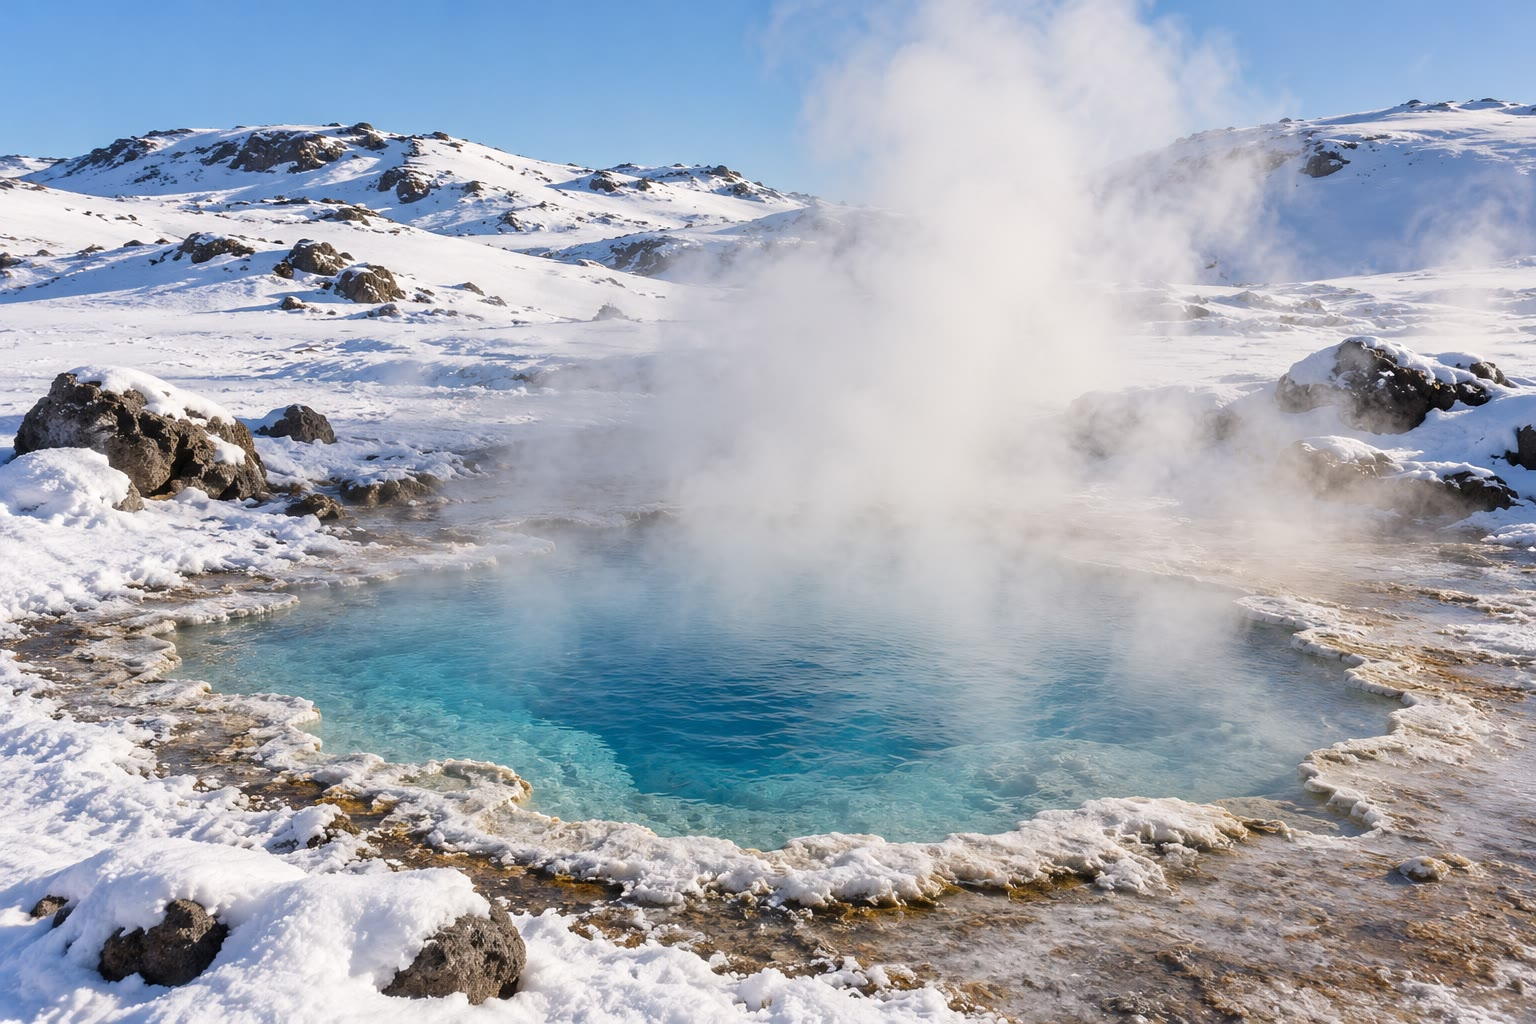
\includegraphics[width=0.6\linewidth]{images/book2/ai/g12-hot-spring-snow.jpg}

{\small Uma fonte termal fumegando numa paisagem nevada: a água aquecida a
grande profundidade volta à superfície. Ilustração gerada por IA.}
\end{omfigure}

\begin{omfigure}
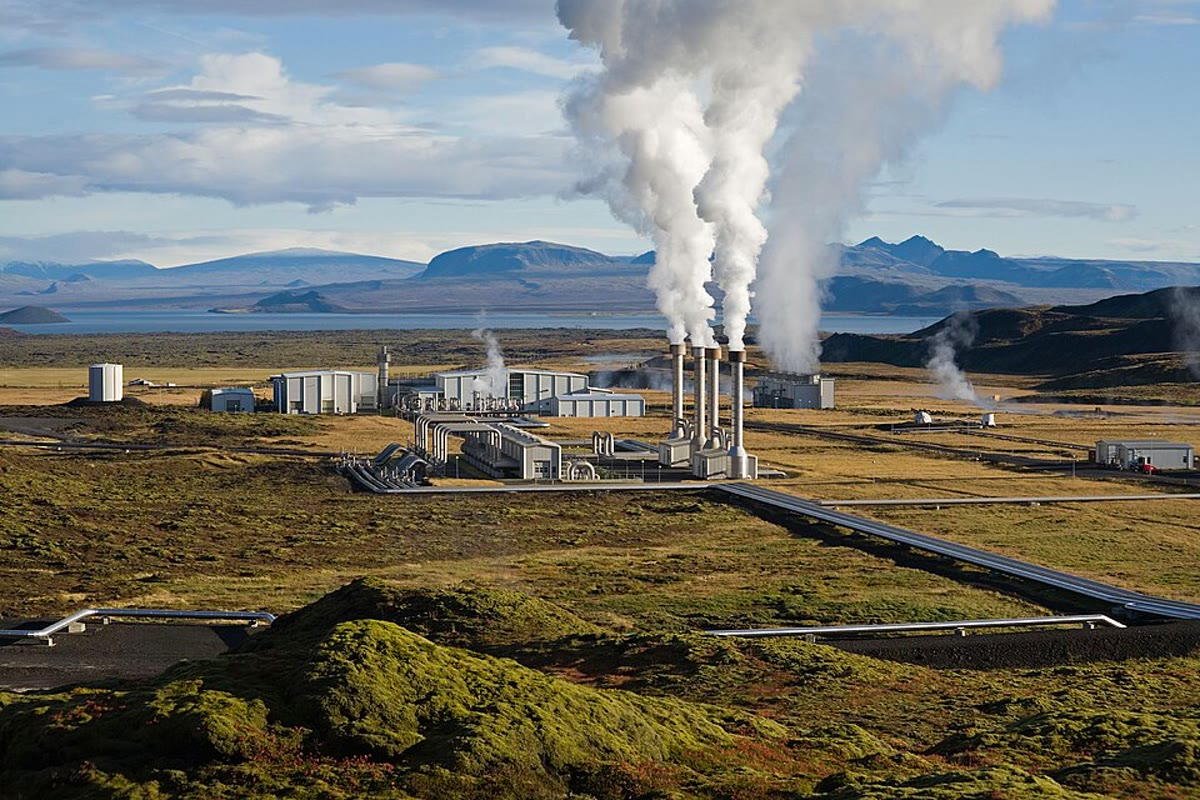
\includegraphics[width=0.66\linewidth]{images/book2/g12-nesjavellir-geothermal.jpg}

{\small A usina geotérmica de Nesjavellir, na área vulcânica de Hengill, na
Islândia: até \qty{120}{MW} de eletricidade e até \qty{300}{MW} de calor,
levados pela água quente. Fotografia Gretar Ívarsson (domínio público).}
\end{omfigure}
% ledger: photo:g12-nesjavellir, on:nesjavellir

Um campo geotérmico não é inesgotável na escala de uma vida humana. Em The
Geysers, na Califórnia, poços demais exploraram o vapor, mais depressa do
que o lento \omterm{def:g12:internal-heat:heat-flow}{fluxo de calor} e a chuva podiam repô-lo: a pressão do vapor caiu
a menos da metade do seu pico, e mais de \qty{40}{\percent} da capacidade
das usinas se perdeu. Hoje, água é injetada de volta no campo para frear o
declínio.
% ledger: cpuc:geysers

\section{Exercícios}

\begin{exercise}[$\star$]\label{exo:g12:internal-heat:1}
Dê a palavra: (a) a potência que sai do interior através de cada metro
quadrado de superfície; (b) o calor liberado pelo decaimento dos átomos
radioativos numa unidade de volume de rocha; (c) a perda do calor armazenado
desde que a Terra se formou; (d) o transporte de calor pelo movimento do
próprio material; (e) o calor interno da Terra usado pelas pessoas.
\end{exercise}

\begin{exercise}[$\star$]\label{exo:g12:internal-heat:2}
Converta: (1) \qty{91.6}{mW/m^2} em \unit{W/m^2}; (2) \qty{46.7}{TW} em
watts; (3) \qty{29}{\celsius} por quilômetro em kelvins por metro.
\end{exercise}

\begin{exercise}[$\star$]\label{exo:g12:internal-heat:3}
Cite os quatro isótopos que produzem quase todo o calor radiogênico, e diga
quais dois o detector KamLAND consegue ver.
\end{exercise}

\begin{exercise}[$\star$]\label{exo:g12:internal-heat:4}
Usando $q = 490/\sqrt{t}$, calcule o \omterm{def:g12:internal-heat:heat-flow}{fluxo de calor} através de um fundo
oceânico de 1, 4, 25 e 49 milhões de anos.
\end{exercise}

\begin{exercise}[$\star$]\label{exo:g12:internal-heat:5}
Por que o \omterm{def:g12:internal-heat:heat-flow}{fluxo de calor} é medido em furos de sondagem e não na própria
superfície? Por que é preciso esperar depois da perfuração antes de medir?
\end{exercise}

\begin{exercise}[$\star\star$]\label{exo:g12:internal-heat:6}
No furo de sondagem KTB, a rocha estava a cerca de \qty{265}{\celsius} a
\qty{9.1}{km}. (1) Tomando \qty{10}{\celsius} na superfície, calcule o
gradiente médio. (2) Com uma condutividade de \qty{2.72}{W/(m.K)}, que \omterm{def:g12:internal-heat:heat-flow}{fluxo
de calor} ele dá? (3) Compare com a média dos continentes.
\end{exercise}

\begin{exercise}[$\star\star$]\label{exo:g12:internal-heat:7}
Os continentes cobrem \qty{2.073e14}{m^2} com um \omterm{def:g12:internal-heat:heat-flow}{fluxo de calor} médio de
\qty{70.9}{mW/m^2}, os oceanos \qty{3.028e14}{m^2} com
\qty{105.4}{mW/m^2}. Calcule a potência perdida por cada um, o total, e a
parte perdida através do fundo oceânico.
\end{exercise}

\begin{exercise}[$\star\star$]\label{exo:g12:internal-heat:8}
Uma camada de \omterm{def:g12:subduction-magmatism:granodiorite}{granodiorito} de \qty{8}{km} de espessura tem uma produção de
calor de \qty{1.88}{\micro W/m^3}. (1) Que \omterm{def:g12:internal-heat:heat-flow}{fluxo de calor} ela produz na
superfície? (2) Que parte de \qty{70.9}{mW/m^2} é isso?
\end{exercise}

\begin{exercise}[$\star\star$]\label{exo:g12:internal-heat:9}
Com que idade o fundo oceânico perde tanto calor quanto o continente médio,
\qty{70.9}{mW/m^2}, segundo $q = 490/\sqrt{t}$?
\end{exercise}

\begin{exercise}[$\star\star$]\label{exo:g12:internal-heat:10}
Quanto mais calor o urânio-235 liberava há 1.4 bilhão de anos do que hoje? E
o potássio-40, há 2.5 bilhões de anos?
\end{exercise}

\begin{exercise}[$\star\star$]\label{exo:g12:internal-heat:11}
Usando $t \approx L^2/\kappa$ com $\kappa = \qty{1e-6}{m^2/s}$, quanto tempo
o calor leva para atravessar por condução (1) um derrame de lava de
\qty{10}{m} de espessura; (2) uma \omterm{def:g11:lithosphere-asthenosphere:lithosphere}{litosfera} de \qty{100}{km} de espessura;
(3) o manto? Expresse cada resultado em unidades sensatas.
\end{exercise}

\begin{exercise}[$\star\star\star$]\label{exo:g12:internal-heat:12}
Hoje, o tório-232 libera cerca de \qty{10.4}{TW}, o urânio-238
\qty{9.6}{TW}, o potássio-40 \qty{4.0}{TW} e o urânio-235 \qty{0.42}{TW}.
Usando as meias-vidas da figura, calcule o calor de cada um há 3 bilhões de
anos, o total, e a parte dos dois isótopos de vida curta.
\end{exercise}

\begin{exercise}[$\star\star\star$]\label{exo:g12:internal-heat:13}
A usina de Nesjavellir pode fornecer até \qty{300}{MW} de calor, levados por
cerca de \qty{1640}{L} de água quente por segundo. Com um calor específico
de \qty{4180}{J/(kg.K)} e uma massa de \qty{1}{kg} por litro, em quantos
graus essa água foi aquecida? Que área de continente médio perde
\qty{300}{MW} de calor?
\end{exercise}

\begin{exercise}[$\star\star\star$]\label{exo:g12:internal-heat:14}
Suponha que uma placa leva 100 milhões de anos para ir de uma dorsal a uma
fossa, e que um circuito de convecção através de todo o manto leva cerca de
200 milhões de anos. (1) Compare esses tempos com os 260 bilhões de anos da
condução através do manto. (2) Por que a convecção pode levar o calor tão
mais depressa, embora o manto se mova só alguns centímetros por ano?
\end{exercise}

\begin{exercise}[$\star\star\star$]\label{exo:g12:internal-heat:15}
Suponha que o núcleo perde cerca de \qty{10}{TW} de calor para o manto
através do \omterm{def:g11:seismic-structure:core}{limite manto--núcleo}, a \qty{2891}{km} de profundidade. (1) Que
parte do \omterm{def:g12:internal-heat:secular-cooling}{resfriamento secular}, \qty{22.3}{TW}, isso seria? De onde vem o
resto? (2) Calcule o \omterm{def:g12:internal-heat:heat-flow}{fluxo de calor} médio através do \omterm{def:g11:seismic-structure:core}{limite manto--núcleo},
e compare-o com o \omterm{def:g12:internal-heat:heat-flow}{fluxo de calor} médio na superfície,
\qty{91.6}{mW/m^2}. (3) Por que o núcleo quente pode aquecer a base do manto
embora o manto seja sólido?
\end{exercise}

\begin{problem}[{Problema de fim de semana --- o balanço de calor da Terra}]
\label{pb:g12:internal-heat:1}
% ledger: b2dd10:continents, b2dd10:half-space, kamland11:geonu, dye12:isotopes, dye12:bse, b2vila:heat-production
% values (internal_heat.py): radiogenic 24.4 TW, secular 22.3 TW, share 0.523, K40 4.0, U235 0.42, U238 9.59
O \omterm{def:g12:internal-heat:heat-flow}{fluxo de calor} da Terra foi medido em mais de 38\,000 lugares. Em média,
os continentes perdem \qty{70.9}{mW/m^2} em \qty{2.073e14}{m^2}, e o fundo
oceânico \qty{105.4}{mW/m^2} em \qty{3.028e14}{m^2}.

\medskip
\noindent\textbf{Parte I --- Fluxo de calor e áreas.}
\begin{enumerate}
  \item Verifique que as duas áreas somam a área de uma esfera de raio
        \qty{6371}{km}.
  \item Que fração da superfície é fundo oceânico?
  \item Por que o fundo oceânico perde mais calor por metro quadrado que os
        continentes?
  \item Usando $q = 490/\sqrt{t}$, calcule o \omterm{def:g12:internal-heat:heat-flow}{fluxo de calor} através de um
        fundo oceânico de 4 milhões de anos.
  \item Um furo de sondagem no granito (\qty{2.72}{W/(m.K)}) mede
        \qty{26}{\celsius} por quilômetro. O seu \omterm{def:g12:internal-heat:heat-flow}{fluxo de calor} fica acima
        ou abaixo da média continental?
\end{enumerate}

\medskip
\noindent\textbf{Parte II --- O total.}
\begin{enumerate}[resume]
  \item Calcule a potência perdida através dos continentes.
  \item Calcule a potência perdida através do fundo oceânico.
  \item Some-as: o \omterm{def:g12:internal-heat:heat-flow}{fluxo de calor} total da Terra, em terawatts.
  \item Qual é o \omterm{def:g12:internal-heat:heat-flow}{fluxo de calor} médio sobre toda a superfície?
  \item Se \qty{10}{km} de granito (\qty{24.3}{mW/m^2}) estivessem sob todos
        os continentes, quantos terawatts eles produziriam? Compare com a
        potência perdida através dos continentes.
\end{enumerate}

\medskip
\noindent\textbf{Parte III --- O calor radiogênico.}
\begin{enumerate}[resume]
  \item O KamLAND conta os geoneutrinos do urânio-238 e do tório-232: juntos,
        eles liberam cerca de \qty{20.0}{TW}, com \qty{3.9}{kg} de tório na
        Terra para cada quilograma de urânio. Um quilograma de urânio libera
        \qty{94.4}{\micro W} pelo seu urânio-238 e \qty{4.10}{\micro W} pelo
        seu urânio-235; um quilograma de tório, \qty{26.3}{\micro W}.
        Calcule o calor do urânio-238, depois o do urânio-235.
  \item O potássio-40 acrescenta cerca de \qty{4}{TW}. Calcule o calor
        radiogênico total.
  \item Que tipo de rocha contém a maior parte desses elementos, e onde ela
        fica?
  \item O calor radiogênico era maior ou menor há 3 bilhões de anos? Por quê?
\end{enumerate}

\medskip
\noindent\textbf{Parte IV --- O resfriamento secular.}
\begin{enumerate}[resume]
  \item Que potência não é fornecida pela radioatividade?
  \item De onde ela vem?
  \item Calcule a parte do \omterm{def:g12:internal-heat:heat-flow}{fluxo de calor} fornecida pelo \omterm{def:g12:internal-heat:secular-cooling}{resfriamento
        secular}.
  \item Os modelos da composição da Terra dão um calor radiogênico de 11 a
        \qty{38}{TW}.
        Entre que partes fica então a parte radiogênica?
  \item O que leva a maior parte desse calor através do manto?
  \item Resuma: que parte da perda de calor da Terra a radioatividade
        fornece hoje?
\end{enumerate}
\end{problem}
